% -----------------------------------------------
% Template for SMC 2022
% based on SMC 2022 template
% -----------------------------------------------

\documentclass{article}

\usepackage{smc}
\usepackage{times}
\usepackage{ifpdf}
\usepackage[english]{babel}
\usepackage{cite}
\usepackage[dvipsnames]{xcolor}
\def\TLcomment[#1]{\textcolor{red}{#1}}
\def\SWcomment[#1]{\textcolor{blue}{#1}}
\def\SScomment[#1]{\textcolor{orange}{#1}}

%%%%%%%%%%%%%%%%%%%%%%%% Some useful packages %%%%%%%%%%%%%%%%%%%%%%%%%%%%%%%
%%%%%%%%%%%%%%%%%%%%%%%% See related documentation %%%%%%%%%%%%%%%%%%%%%%%%%%
\usepackage{amsmath} % popular packages from Am. Math. Soc. Please use the 
\usepackage{amssymb} % related math environments (split, subequation, cases,
\usepackage{amsfonts}% multline, etc.)
%\usepackage{bm}      % Bold Math package, defines the command \bf{}
%\usepackage{paralist}% extended list environments
%%subfig.sty is the modern replacement for subfigure.sty. However, subfig.sty 
%%requires and automatically loads caption.sty which overrides class handling 
%%of captions. To prevent this problem, preload caption.sty with caption=false 
%\usepackage[caption=false]{caption}
%\usepackage[font=footnotesize]{subfig}

\def\ctxt{\text{c}} %connection subscript (text)
\def\stxt{{\text{s}}} %string subscript (text)
\def\ptxt{\text{p}} %plate subscript (text)
\def\mtxt{\text{m}} %mass subscript (text)
\def\itxt{\text{i}} %point of 'interest' subscript (text)
\def\Btxt{\text{B}} %bow subscript (text)
\def\etxt{\text{e}} %excitation subscript (text)
\def\rtxt{\text{r}} %lip reed subscript (text)
\def\ttxt{\text{t}} %tube subscript (text)


\def\sgn{\text{sgn}}
\def\sm{\text{sm}} %string-mass interaction tromba
\def\mp{\text{mp}} %mass-plate interaction tromba

\def\MoneD{{\mathcal{M}^n}}
\def\MtwoD{{\mathcal{M}_2^n}}

\def\Nfrac{\mathcal{N}}
\def\flip{\leftarrow}
\def\Ucal{\mathbfcal{U}}

% states
\def\uln{u_l^n}
\def\wln{w_l^n}
\def\wmn{w_m^n}
\def\un{u^n}
\def\ulmn{u_{l,m}^n}
\def\ulm{u_{l,m}}
\def\uqn{u_q^n}
\def\qlmn{q_{l,m}^n}

\def\wlmn{w_{l,m}^n}
\def\zlmn{z_{l,m}^n}
\def\ubr{u_\text{br}}
\def\zbr{z_\text{br}}

\def\qln{q_l^n}
\def\lv{{l_v}}
\def\lw{{l_w}}
\def\vlvn{v_\lv^n}
\def\ulcn{u_{l_\ctxt}^n}
\def\wlwn{w_\lw^n}
\def\wmcn{w_{m_\ctxt}^n}

\def\wmn{w_m^n}

\def\Psiln{\Psi_l^n}
\def\Psinp{\Psi_l^{n+1}}
\def\Psinm{\Psi_l^{n-1}}
\def\Psilp{\Psi_{l+1}^n}
\def\Psilm{\Psi_{l-1}^n}

% bold symbols (state vectors and matrices)
\def\u{\mathbf{u}}
\def\w{\mathbf{w}}
\def\ww{\boldsymbol{w}}
\def\q{\mathbf{q}}
\def\v{\mathbf{v}}
\def\vv{\boldsymbol{v}}
\def\z{\mathbf{z}}
\def\Z{\mathbf{Z}}
\def\I{\mathbf{I}}
\def\A{\mathbf{A}}
\def\B{\mathbf{B}}
\def\C{\mathbf{C}}
\def\Q{\mathbf{Q}}
\def\U{\mathbf{U}}
\def\J{\mathbf{J}}
\def\i{\mathbf{i}}
\def\j{\mathbf{j}}
\def\BB{\mathbfcal{B}^n}


% interpolators
\def\Iu{I_{l, u}(x_\ctxt)}
\def\Iw{I_{m, w}(\chi_\ctxt)}
\def\Ju{J_{l, u}(x_\ctxt)}
\def\Jw{J_{m, w}(\chi_\ctxt)}
\def\Iq{I_q(\chi_\ctxt)}
\def\Ilm{I_{l,m}(x_\ctxt)}

\def\uStack{\boldsymbol{u}}
\def\qq{\boldsymbol{q}}

% mathfraks
\def\H{\mathfrak{H}}
\def\h{\mathfrak{h}}
\def\t{\mathfrak{t}}
\def\b{\mathfrak{b}}
\def\p{\mathfrak{p}}
% continuous operators
\def\ptt{\partial_t^2} 
\def\pxx{\partial_x^2}
\def\pxxx{\partial_x^3}
\def\pxxxx{\partial_x^4}
\def\pcc{\partial_{\chi}^2}
\def\pcccc{\partial_{\chi}^4}

\def\pyy{\partial_y^2}

\def\pt{\partial_t} 
\def\px{\partial_x} 
\def\py{\partial_y} 

% discrete operators
\def\dtt{\delta_{tt}} 
\def\dxx{\delta_{xx}}
\def\dxxx{\delta_{xxx}}
\def\dxxxx{\delta_{xxxx}}
\def\dcc{\delta_{\chi\chi}}
\def\dcccc{\delta_{\chi\chi\chi\chi}}

\def\dtd{\delta_{t\cdot}} 
\def\dtp{\delta_{t+}} 
\def\dtm{\delta_{t-}} 

\def\dxd{\delta_{x\cdot}} 
\def\dxp{\delta_{x+}} 
\def\dxm{\delta_{x-}} 
\def\dyd{\delta_{y\cdot}} 
\def\dyp{\delta_{y+}} 
\def\dym{\delta_{y-}} 

\def\mtt{\mu_{tt}} 
\def\mtd{\mu_{t\cdot}} 
\def\mtp{\mu_{t+}} 
\def\mtm{\mu_{t-}} 

\def\mxx{\mu_{xx}} 
\def\mxd{\mu_{x\cdot}} 
\def\mxp{\mu_{x+}} 
\def\mxm{\mu_{x-}} 

\def\dDelta{\delta_{\Delta}}
% \def\dDbox{\delta_{\Delta\boxplus}}
\def\dyy{\delta_{yy}}

% matrix operators
\def\Dxx{\mathbf{D}_{xx}}
\def\Dyy{\mathbf{D}_{yy}}
\def\DDxx{\mathbfcal{D}_{xx}^n}
\def\DDyy{\mathbfcal{D}_{yy}^n}
\def\Dxxxx{\mathbf{D}_{xxxx}}
\def\DDxxxx{\mathbfcal{D}_{xxxx}^n}

\def\DDeltamat{\mathbf{D}_\Delta}
\def\DDeltaDelta{\mathbf{D}_{\Delta\Delta}}
\def\DDDelta{\mathbfcal{D}_{\Delta}^n}
\def\DDDeltaDelta{\mathbfcal{D}_{\Delta\Delta}^n}

\def\Mv{M_v^n}
\def\Mw{M_w^n}

% often-used variables
\def\sz{\sigma_{0}}
\def\so{\sigma_{1}}
\def\vrel{v_\text{rel}}
\def\Sbar{\bar{S}}
\def\Sm{S_{l-1/2}}
\def\Sp{S_{l+1/2}}

\def\szX[#1]{\sigma_{0,{#1}}}
\def\soX[#1]{\sigma_{1,{#1}}}

\def\fs{f_\text{s}}
\def\el{\epsilon_\text{l}}
\def\er{\epsilon_\text{r}}
% mathcals
\def\D{\mathcal{D}}
\def\L{\mathcal{L}}
\def\OO{\mathcal{O}}
\def\S{\mathcal{S}}

% flooring ceiling
\def\floor[#1]{\left\lfloor #1 \right\rfloor}
\def\ceil[#1]{\left\lceil #1 \right\rceil}
\def\ansatz{\ \overset{\mathcal{A}}{\Longrightarrow}\ }
% other
\def\qaq{\quad \text{and} \quad}
\def\qwiq{\quad \text{with} \quad}
\def\qwhq{\quad \text{where} \quad}

\def\mystrut{\rule[-.2\baselineskip]{0pt}{\baselineskip}}

\def\th{\textsuperscript{th} }
\def\thOrder{\textsuperscript{th}-order }

\def\boldPhi{\boldsymbol{\phi}}
\def\boldPsi{\boldsymbol{\Psi}}
\def\eig{\text{eig}}

\def\Dxx{\mathbf{D}_{xx}}
\def\alf{'}
\def\DxxA{\Dxx\alf}
\def\DyyA{\Dyy\alf}
\def\DxxxxA{\Dxxxx\alf}
\def\DDeltamatA{\DDeltamat\alf}
\def\DDeltaDeltaA{\DDeltaDelta\alf}
\def\Aterm{\mathcal{I}^n}


\def\AA{\mathbfcal{A}^n}
\def\BB{\mathbfcal{B}^n}
\def\CC{\mathbfcal{C}^n}

\DeclareMathAlphabet{\mathcal}{OMS}{ntxsy}{m}{n}   % or txsy
\DeclareMathAlphabet\mathbfcal{OMS}{cmsy}{b}{n} % for paper A

% \makeatletter
% \renewcommand*\env@matrix[1][*\c@MaxMatrixCols c]{%
%   \hskip -\arraycolsep
%   \let\@ifnextchar\new@ifnextchar
%   \array{#1}}
% \makeatother
% \usepackage{tabstackengine}
% \stackMath


%user defined variables
\def\papertitle{Modular Physical Models in a Real-Time Interactive Application}
\def\firstauthor{Silvin Willemsen}
\def\secondauthor{Titas Lasickas}
\def\thirdauthor{Stefania Serafin}

% adds the automatic
% Saves a lot of output space in PDF... after conversion with the distiller
% Delete if you cannot get PS fonts working on your system.

% pdf-tex settings: detect automatically if run by latex or pdflatex
\newif\ifpdf
\ifx\pdfoutput\relax
\else
   \ifcase\pdfoutput
      \pdffalse
   \else
      \pdftrue
\fi

\ifpdf % compiling with pdflatex
  \usepackage[pdftex,
    pdftitle={\papertitle},
    pdfauthor={\firstauthor, \secondauthor, \thirdauthor},
    bookmarksnumbered, % use section numbers with bookmarks
    pdfstartview=XYZ % start with zoom=100% instead of full screen; 
                     % especially useful if working with a big screen :-)
   ]{hyperref}
  %\pdfcompresslevel=9

  \usepackage[pdftex]{graphicx}
  % declare the path(s) where your graphic files are and their extensions so 
  %you won't have to specify these with every instance of \includegraphics
  \graphicspath{{./figures/}}
  \DeclareGraphicsExtensions{.pdf,.jpeg,.png}

  \usepackage[figure,table]{hypcap}

\else % compiling with latex
  \usepackage[dvips,
    bookmarksnumbered, % use section numbers with bookmarks
    pdfstartview=XYZ % start with zoom=100% instead of full screen
  ]{hyperref}  % hyperrefs are active in the pdf file after conversion

  \usepackage[dvips]{epsfig,graphicx}
  % declare the path(s) where your graphic files are and their extensions so 
  %you won't have to specify these with every instance of \includegraphics
  \graphicspath{{./figures/}}
  \DeclareGraphicsExtensions{.eps}

  \usepackage[figure,table]{hypcap}
\fi

%setup the hyperref package - make the links black without a surrounding frame
\hypersetup{
    colorlinks,%
    citecolor=black,%
    filecolor=black,%
    linkcolor=black,%
    urlcolor=black
}


% Title.
% ------
\title{\papertitle}

% Authors
% Please note that submissions are NOT anonymous, therefore 
% authors' names have to be VISIBLE in your manuscript. 
%
% Single address
% To use with only one author or several with the same address
% ---------------
%\oneauthor
%   {\firstauthor} {Affiliation1 \\ %
%     {\tt \href{mailto:author1@smcnetwork.org}{author1@smcnetwork.org}}}

%Two addresses
%--------------
% \twoauthors
%   {\firstauthor} {Affiliation1 \\ %
%     {\tt \href{mailto:author1@smcnetwork.org}{author1@smcnetwork.org}}}
%   {\secondauthor} {Affiliation2 \\ %
%     {\tt \href{mailto:author2@smcnetwork.org}{author2@smcnetwork.org}}}

% Three addresses
% --------------
 \oneauthor
   {\firstauthor, \secondauthor, and \thirdauthor} {Multisensory Experience Lab, CREATE,\\
   Aalborg University Copenhagen, Denmark \\ %
     {\tt \href{mailto:sil@create.aau.dk}{sil@create.aau.dk}}}


% ***************************************** the document starts here ***************
\begin{document}
%
\capstartfalse
\maketitle
\capstarttrue
%
\begin{abstract}
Through recent advances in processing power, physical modelling using finite-difference time-domain (FDTD) methods has gained popularity. Many different musical instrument models based on these methods exist, and nearly all are based on the same underlying systems and interactions between them. This paper presents an application where individual resonator modules, such as strings, bars, membranes and plates, can be connected in a modular fashion and interacted with in real time. Various excitations, including the bow, hammer and pluck, are implemented as well, allowing for expressive control and a wide sonic palette. Existing and non-existing model configurations can easily be implemented, modified and experimented with, as well as the parameters describing them.
%Due to their generality, these methods lend themselves to a modular framework where various existing models can be connected in arbitrary ways. 
\end{abstract}
%

\section{Introduction}\label{sec:introduction}
Any acoustic musical instrument can be subdivided into a resonator and exciter component \cite{Borin1989}. Examples of resonator-exciter combinations are the violin and the bow, and the guitar and the pick. Many resonators, such as those mentioned here, can be further subdivided into basic components, i.e., a set of individual strings, a bridge and a wooden body. As many instruments consist of the same basic resonators -- simply with different geometries or made from different materials -- one can imagine some application that can implement many musical instruments based on the same fundamental resonator components in a modular fashion. Using physical modelling to implement these resonators allows for accurate implementation of the resonators, as well as the interactions between them.  

Modularity in physical modelling sound synthesis is by no means a new concept. The earliest example of a modular system for sound synthesis was due to Cadoz \textit{et al.} \cite{Cadoz1983}, with the CORDIS system that allows complex instruments to be created using simple mass-spring systems. Later, Morrison and Adrien created Mosaic \cite{Morrison1993}, a modular environment using modal synthesis \cite{Adrien1991}. Rabenstein \textit{et al.} presented modular physical models with a block-based approach using wave digital filters \cite{Rabenstein2007} and digital waveguides \cite{Smith1992}. 

Finite-difference time-domain (FDTD) methods, first used in a musical context by Ruiz \cite{Ruiz1969}, Hiller and Ruiz \cite{Hiller1971I, Hiller1971II} and later by Chaigne \cite{Chaigne1992}, also lend themselves to modularity. In \cite{Bilbao2009Modular}, Bilbao presents a modular environment where bars and plates are connected by nonlinear springs, and in \cite{Bilbao2014} Bilbao \textit{et al.} propose a modular environment including higher dimensional systems.

Due to recent increase in computational power, FDTD methods have gained popularity in real-time applications \cite{WillemsenThesis}. A real-time modular environment using strings and lumped objects is presented in \cite{Bilbao2019}, and a real-time implementation of connected strings and bars using the FAUST programming language due to S\"udholt \textit{et al.} in \cite{Sudholt2021}. 

The main goal of the aforementioned literature on FDTD-based modular environments is to create arbitrary sound-generators based on physical equations of motion, rather than modelling existing instruments. Furthermore, those able to run in real time only include systems spatially distributed over a maximum of one dimension. Many instruments require higher-dimensional structures to more accurately reproduce their sound. As done in e.g. \cite{Willemsen2019, Willemsen2020}, the body of stringed instruments can be simplified to a thin plate, which is a system distributed over two dimensions. 

This work presents an interactive modular environment in a real-time application where FDTD implementations of strings, bars, membranes and plates can be connected and played by the user. Although it is still possible to create arbitrary configurations to build non-existing instruments, the focus of this contribution is to allow for the possibility of modelling existing instruments. The current work aims to generalise previous work done on musical instruments modelled using FDTD methods (see e.g. \cite{Willemsen2019, Willemsen2020, Lasickas2021, Sudholt2021Langeleik, Mosen2021}), such that these can all be easily implemented as `presets' of a modular application. As many of these instruments consist of the same components, one can avoid from-the-ground-up implementation in the future. This work is part of a larger project, which will see its fruition in virtual reality (VR), where it will be used as a sound engine.

The rest of this paper is structured as follows: Section \ref{sec:models} describes the physical models used in this work, including resonators, exciters and connections between resonators and Section \ref{sec:discrete} describes how to implement these. Section \ref{sec:application} presents the functionality of the real-time application, Section \ref{sec:resDiscuss} presents results and discusses these, and concluding remarks appear in Section \ref{sec:conclusion}.

\section{Models}\label{sec:models}
This section describes the continuous-time equations of the systems used in the application. Consider a state variable $q(\boldsymbol{x}, t)$ with time $t\geq 0$ (in s) and spatial coordinate $\boldsymbol{x}\in \mathcal{D}$, where the dimensions and definition of domain $\mathcal{D}$ depend on the system at hand. The dynamics of a system can then be written using the following general form:
\begin{equation}\label{eq:generalForm}
    \mathcal{L}q = 0,
\end{equation}
where linear partial differential operator $\mathcal{L}$ describes the dynamics of a model in isolation.

This section presents the partial differential equations (PDEs) of the stiff string and the stiff membrane. These can be used as a general equation for modelling other 1D and 2D systems respectively through a special choice of parameters. 

% The output of any model can be obtained by listening to $q(\boldsymbol{x}_\text{o}, t)$ for an output location $\boldsymbol{x}_\text{o} \in \mathcal{D}$. 

\subsection{1D Systems}
A commonly used 1D model (see e.g. \cite{Willemsen2019, Bilbao2019}) is the damped stiff string (or string for short). With reference to Eq. \eqref{eq:generalForm}, consider a string of length $L$ (in m), its transverse displacement described by state variable $q = u(\chi, t)$ (in m), and spatial coordinate $\chi$ is defined over domain $\mathcal{D} = [0, L]$. Furthermore, $\mathcal{L}=\mathcal{L}^{(\text{1})}$ is defined as \cite{Bensa2003}
% \begin{equation}\label{eq:stiffString}
%     \mathcal{L}_\stxt = \rho_\stxt A\ptt - T_\stxt \pcc + E_\stxt I \pcccc + 2\szX[\stxt]\rho_\stxt A\pt - 2 \soX[\stxt]\rho_\stxt A\pt\pcc,
% \end{equation}
\begin{equation}\label{eq:stiffString}
    \mathcal{L}^{(1)}= \rho A\ptt - T\pcc + E I \pcccc + 2\sz\rho A\pt - 2 \so\rho A\pt\pcc,
\end{equation}
where $\pt$ and $\partial_\chi$ denote partial differentiation with respect to time and space respectively. The model is parameterised by material density $\rho$ (in kg/m$^3$), cross-sectional area $A = \pi r^2$ (in m$^2$), radius $r$ (in m), tension $T$ (in N), Young's modulus $E$ (in Pa), area moment of inertia $I = \pi r^4/4$ (in m$^4$) and loss coefficients $\sz$ (in s$^{-1}$) and $\so$ (in m$^2$/s). If $T=0$, the model reduces to a damped bar. Note that a circular cross-section is assumed here. Finally, in this work, the boundary conditions are chosen to be simply supported as
\begin{equation}
    u = \pcc u = 0, \quad \text{for}, \quad \chi = 0, L.
\end{equation}

\subsection{2D Systems}
An often-used 2D system is the thin plate (see e.g. \cite{Webb2015, Willemsen2020}). However, to retain generality, and the possibility to model membranes a well, the PDE for a stiff membrane will be presented here.

Consider a rectangular stiff membrane (or membrane for short) with side lengths $L_x$ and $L_y$ (both in m). With reference to Eq. \eqref{eq:generalForm} its transverse displacement can be described by $q = w(x, y, t)$ (in m), which is defined for domain
$\mathcal{D} = [0, L_x] \times [0, L_y]$, and $\mathcal{L}=\mathcal{L}^{(2)}$ is defined as \cite{Fletcher1998}
% \begin{equation}\label{eq:stiffMembrane}
%     \begin{aligned}
%         \mathcal{L}_\ptxt = &\ \rho_\ptxt H\ptt - T_\ptxt \Delta + D \Delta\Delta+ 2\szX[\ptxt]\rho_\ptxt H\pt \\
%         & - 2 \soX[\ptxt]\rho_\ptxt H\pt\Delta.
%     \end{aligned}
% \end{equation}
\begin{equation}\label{eq:stiffMembrane}
        \mathcal{L}^{(2)} = \rho H\ptt - T \Delta + D \Delta\Delta+ 2\sz\rho H\pt - 2 \so\rho H\pt\Delta,
\end{equation}
Here, $\Delta = \pxx + \pyy$ is the Laplacian, and parameters are material density $\rho$ (in kg/m$^3$), thickness $H$ (in m), tension per unit length $T$ (in N/m), stiffness coefficent $D = E H^3 / 12 (1-\nu^2)$ (in kg $\cdot$ m$^2\cdot$s$^{-2}$), Young's modulus $E$ (in Pa), dimensionless Poisson's ratio $\nu$, and loss coefficients $\sz$ (in s$^{-1}$) and $\so$ (in m$^2$/s).
If $T = 0$, the model reduces to a thin plate, and if $D=0$ it reduces to the 2D wave equation, which can be used to model a non-stiff membrane.
%
For simplicity, boundary conditions are chosen to be clamped, such that
\begin{equation}
        w = {\bf n} \cdot \nabla w = 0,
\end{equation}
where $\nabla$ denotes `the gradient of', and ${\bf n}$ is a normal to the plate area at the boundary.

\subsection{Connections}\label{sec:contConnections}
% is characterised by 

% Following the notation in \cite{Sudholt2021}, a connection

One can add connections between instances of the models presented above by extending the general form in Eq. \eqref{eq:generalForm}. Consider $M$ models $q_m$ indexed by $m \in \mathfrak{M}$, where $\mathfrak{M} = \{1, \hdots, M\}$ and $C$ connections between them. A connection is indexed by $c\in \mathfrak{C}$ with $\mathfrak{C} = \{1, \hdots, C\}$, and is characterised by the indices of the models it connects -- $r_c \in \mathfrak{M}$ and $s_c\in \mathfrak{M}$ -- and the locations where these models are connected -- $\boldsymbol{x}_{r, c}\in \mathcal{D}_{r_c}$ and $\boldsymbol{x}_{s, c}\in \mathcal{D}_{s_c}$. Here, domains $\mathcal{D}_{r_c}$ and $\mathcal{D}_{s_c}$ are the (spatial) domains that models $q_{r_c}$ and $q_{s_c}$ are defined for.  

Model $q_{r_c}$ will be placed `below' $q_{s_c}$ such that the connection force acts positively on the former and negatively on the latter. The general form in Eq. \eqref{eq:generalForm} can then be extended to include connections according to
% A connection between models $q_{r_c}$ and $q_{s_c}$ where model indices $r_c \in \mathfrak{M}$ and $s_c\in \mathfrak{M}$ is indexed by $c \in \mathfrak{C}$, with $\mathfrak{C} = \{1, \hdots, C\}$. Apart from the models it connects between 
%  at locations $\boldsymbol{x}_{r, c} \in \mathcal{D}_{r_c}$, and $\boldsymbol{x}_{s, c} \in \mathcal{D}_{s_c}$ respectively, can be described by the following 4-tuple $(r_c, s_c, \boldsymbol{x}_{r, c}, \boldsymbol{x}_{s, c})$. Here, model $q_r$ is placed `below' model $q_s$, such that the connection force acts positively on the former and negatively on the latter.  The general form in Eq. \eqref{eq:generalForm} can then be extended to include connections according to
\begin{equation}\label{eq:generalFormConnections}
    \!\!\!\mathcal{L}_mq_m =\!\sum_{\substack{c\in \mathfrak{C}\vspace{0.1em}\\ r_c = m}}\!\! \delta(\boldsymbol{x}_m - \boldsymbol{x}_{r, c}) f_c-\!\! \sum_{\substack{c\in \mathfrak{C}\vspace{0.1em}\\ s_c = m}}\!\! \delta(\boldsymbol{x}_m - \boldsymbol{x}_{s,c}) f_c,
\end{equation}
where $f_c = f_c(t)$ is the force (in N) of the $c$\textsuperscript{th} connection.

The simplest connection considered in this work is the rigid connection, which assumes that the connected systems have an identical displacement at their respective connection locations. Alternatively, as done in \cite{theBible, Bilbao2009Modular}, one can use a spring to connect two systems. A connection force due to a nonlinear damped spring is
\begin{equation}\label{eq:nonlinearSpring}
    f_\ctxt = K_{1, c}\eta_c + K_{3, c}\eta_c^3 + R_c\pt \eta_c,
\end{equation}
with is a linear spring coefficient $K_{1, c}$ (in N/m),  nonlinear spring coefficient $K_{3, c}$ (in N/m$^3$), and damping coefficient $R_c$ (in s$^{-1}$) of the $c$\textsuperscript{th} connection. If $K_{3, c} = 0$, Eq. \eqref{eq:nonlinearSpring} reduces to a linear spring. Furthermore, $\eta_c = \eta_c(t) = q_{s_c}(\boldsymbol{x}_{s,c} ,t) - q_{r_c}(\boldsymbol{x}_{r,c} ,t)$ is the relative displacement of the two systems at their respective connection locations (in m). %\footnote{If the string would be placed above the membrane, $\eta(t) = u(\chi_\ctxt t) - w(x_\ctxt, y_\ctxt, t)$.} 
Section \ref{sec:discConnections} will elaborate on how to calculate the connection forces for all cases in discrete time.

% The general form in Eq. \eqref{eq:generalForm} can be extended to include forces due to connections between systems according to
% \begin{equation}
% \begin{aligned}
%     \mathfrak{C} = \Big\{\big(1, 2, 0.25, 0.25\big), \\
%     \big(1, 2, 0.5, 0.75\big)\Big\}
% \end{aligned}
% \end{equation}
% % \begin{equation}\label{eq:generalFormConnections}
% % \begin{aligned}
% %     \mathcal{L}^{(1)}q^{(1)} &= \sum_i \delta(\boldsymbol{x}^{(1)} - \boldsymbol{x}^{(1)}_{\ctxt, i})f_{\ctxt, i},\\
% %     \mathcal{L}^{(2)}q^{(2)}&= -\sum_i \delta(\boldsymbol{x}^{(2)} - \boldsymbol{x}^{(2)}_{\ctxt, i})f_{\ctxt, i},
% % \end{aligned}
% % \end{equation}
% where $f_{\ctxt, i}$ is the connection force (in N) of the $i$\textsuperscript{th} connection of system $q$ and the spatial Dirac delta function $\delta(\boldsymbol{x}-\boldsymbol{x}_{\ctxt, i})$ locates the effect of the connection to a single location $\boldsymbol{x}_{\ctxt, i}\in \mathcal{D}$.
  
  
To illustrate, consider two models ($M=2$), a string and a membrane, such that $q_1 = u(\chi ,t)$ and $q_2 = w(x,y,t)$, and a single connection between them ($C = 1$) at unspecified locations $\chi_\ctxt \in \mathcal{D}_{s_1}$ and $(x_\ctxt, y_\ctxt) \in \mathcal{D}_{r_1}$ respectively. See Figure \ref{fig:snapshot}. Placing the string above the membrane, we get that $s_1 = 1$ and $r_1 = 2$, i.e., the `above' model of connection $1$ has index $1$, and the `below' model of connection $1$ has index $2$. Substituting the partial differential operators for the string and membrane found in Eqs. \eqref{eq:stiffString} and \eqref{eq:stiffMembrane} respectively, Eq. \eqref{eq:generalFormConnections} becomes, for the string and the membrane respectively
\begin{subequations}
\begin{align}\label{eq:contStringMembraneConn}
        \mathcal{L}^{(1)} u &= -\delta(\chi - \chi_\ctxt)f_1,\\
        \mathcal{L}^{(2)} w &= \delta(x - x_\ctxt, y-y_\ctxt)f_1.
\end{align}
\end{subequations}
% where $\chi_\ctxt$ and $(x_\ctxt, y_\ctxt)$ are the respective connection locations along the string, and on the membrane. The connection force is denoted by $f_\ctxt$ (in N) and has an equal and opposite effect on the string and membrane respectively. It is important to take note of the relative location of the two connected systems, i.e., whether a system is placed `above' or `below' the other as this will determine the signs of the connection forces in Eq. \eqref{eq:contStringMembraneConn}. In this case, the string is placed above the membrane. 

One can apply a rigid connection to Eq. \eqref{eq:contStringMembraneConn} according to \cite{theBible}: 
\begin{equation}
    u(\chi_\ctxt, t) = w(x_\ctxt, y_\ctxt, t).
\end{equation} 
%
If instead a spring connection is chosen,
\begin{equation}
    f_1 = K_{1, 1}\eta_1 + K_{3, 1}\eta_1^3 + R_1\pt \eta_1,
\end{equation}
with $\eta_1 = \eta_1(t) = u(\chi_c, t) - w(x_c, y_c, t)$.

\subsection{Excitations}\label{sec:contExcitations}
In this work, as excitations will only be applied to 1D systems, the state variable of the stiff string, $u(\chi, t)$ will be used for the presentation of the various excitations. For the string, the general form in Eq. \eqref{eq:generalForm}
can thus be extended to (ignoring connections for now)
\begin{equation}\label{eq:generalFormString}
    \mathcal{L}^{(1)} u = e_\etxt f_\etxt,
\end{equation}
where $e_\etxt = e_\etxt(\chi)$ is an excitation distribution and $f_\etxt = f_\etxt(t)$ is the externally supplied excitation force (in N).

\subsubsection{The Bow}
As done in previous work, see e.g. \cite{Willemsen2019}, one can include a bowing interaction by introducing a static friction model. With reference to Eq. \eqref{eq:generalFormString}, the excitation force can be defined using the following friction model \cite{theBible}
\begin{equation}\label{eq:bowForce}
    f_\text{e} = - f_\Btxt\sqrt{2a_\Btxt}\vrel e^{-a_\Btxt\vrel^2+1/2},
\end{equation}
with externally supplied bow force $f_\Btxt = f_\Btxt(t)$ (in N), dimensionless free parameter $a_\Btxt$ and 
\begin{equation}\label{eq:vrel}
    \vrel = \pt u(\chi_\Btxt, t) - v_\Btxt
\end{equation}
is the relative velocity (in m/s) between the string at externally supplied bowing location $\chi_\Btxt = \chi_\Btxt(t)$ (in m) and the externally supplied bow velocity $v_\Btxt = v_\Btxt(t)$ (in m/s).
Furthermore, the excitation distribution is set to be a single point along the string:
\begin{equation}\label{eq:bowDistribution}
    e_\text{e} = \delta(\chi - \chi_\Btxt).
\end{equation}

\subsubsection{Hammer}
Another way of exciting a system is to use a hammer, which can be modelled as a simple mass-spring system. The interaction between the hammer and the string is then modelled as a collision, using the following collision potential \cite{Hertz1881}:
\begin{equation}\label{eq:potential}
    \phi(\eta_\etxt) = \frac{K_\etxt}{\alpha_\etxt+1}[\eta_\etxt]_+^{\alpha_\etxt+1},
\end{equation}
with collision stiffness $K_\etxt \geq 0$ (in N/m$^{\alpha_\etxt}$) and nonlinear collision coefficient $\alpha_\etxt \geq 1$. Furthermore, 
\begin{equation}
    [\eta_\etxt]_+ = 0.5 (\eta_\etxt + |\eta_\etxt|)
\end{equation} 
describes the `positive part of $\eta_\etxt$' and
\begin{equation}
    \eta_\etxt = \eta_\etxt(t) = \theta\big(u(\chi_\etxt, t) - z(t)\big)
\end{equation}
is the relative displacement between the string at collision location $\chi_\etxt$ (in m) and the hammer (in m). Here, $\theta = \tau$ if the string should be excited from above, and $\theta = -\tau$ if it should be excited from below, where $\tau = 1$ if the hammer interaction is triggered and $\tau = 0$ if not.  

Using a change of variables based on energy quadratisation presented in \cite{Ducceschi2021}, one can rewrite the collision potential as
\begin{equation}
    f_\text{e} = -\theta\psi \psi',
\end{equation}
where $\psi = \psi(\eta) = \sqrt{2\phi}$, and using dots to denote a temporal derivative, $\psi' = \dot \psi / \dot \eta$. This change of variables ultimately allows for an explicit implementation of the nonlinear collision. 

Using state variable $z = z(t)$ describing the displacement of the hammer from its equilibrium position (in m), its dynamics, including the collision with the string, can be described by the following PDE:
\begin{equation}\label{eq:massSpring}
    M_\text{z}\ptt z = -K_\text{z} \Big(z - (1-\tau)z_\text{off}\Big) + \theta \psi\psi',
\end{equation}
with mass $M_\text{z}$ (in kg), spring constant $K_\text{z}$ (in N/m) and $z_\text{off} = z_\text{off}(t)$ is an externally supplied offset (in m) (also see \cite{Willemsen2020}). The offset is used to keep the mass away from the equilibrium (and thus the system it excites) when controlling the application without wanting to excite the system. If the hammer excitation is triggered, and thus $\tau = 1$, the offset will no longer have an effect on the mass. The spring force then pulls the hammer towards the system, colliding with it in the process. After the collision, $\tau = 0$, and the offset will affect the mass again to avoid continuous collision between the hammer and the system. 

Finally, with reference to Eq. \eqref{eq:generalFormString}, the excitation distribution is set to be a raised cosine with centre location $\chi_\etxt$ and excitation width $e_\text{w}$ (in m):
\begin{equation}\label{eq:raisedCos}
    e_\etxt(\chi) = \begin{cases}
        \frac{1 - \cos\left(\frac{2\pi (\chi - \chi_\etxt)}{e_\text{w}} + \pi\right)}{2},&\!\!\!\!\text{if}\ \chi_\etxt - \frac{e_\text{w}}{2}\leq \chi \leq \chi_\etxt + \frac{e_\text{w}}{2},\\
        0,& \!\!\!\!\text{otherwise.}
        \end{cases}
\end{equation}
% \begin{equation}\label{eq:raisedCosCont}
%     e_\text{rc}(\chi) = 
%     \begin{cases}
%         \frac{1}{2}\left(1 - \cos\left(\frac{2\pi (\chi - \chi_\etxt - e_\text{w})}{e_\text{w}}\right)\right), & \text{if } \chi_\etxt - e_\text{w}/2\leq \chi \leq \chi_\etxt + e_\text{w}/2,\\
%         0, & \text{otherwise},
%     \end{cases}
% \end{equation}
Note that $\chi_\etxt $ and $e_\text{w}$ must be chosen such that $\chi_\etxt - \frac{e_\text{w}}{2}\in \mathcal{D}$ and $\chi_\etxt + \frac{e_\text{w}}{2} \in \mathcal{D}$, where $\mathcal{D}$ is the domain of the excited system.
\begin{figure}[t]
    \centering
    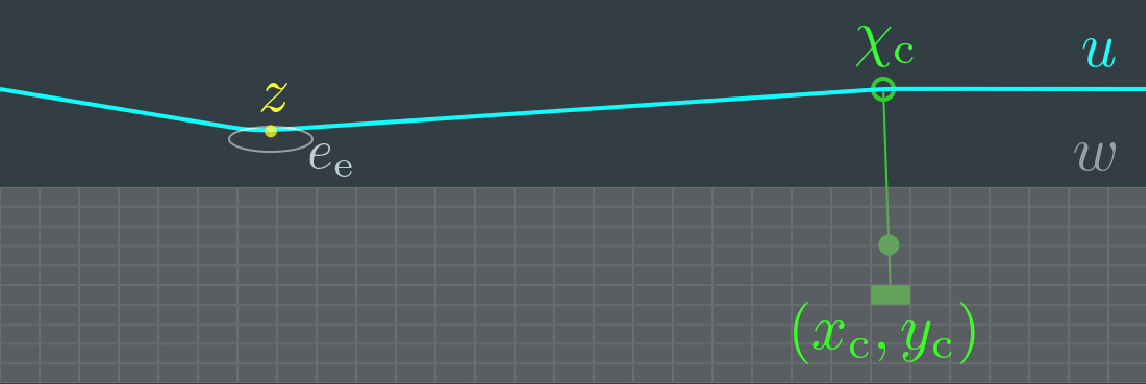
\includegraphics[width = \columnwidth]{snapshot.pdf}
    \caption{Snapshot of the application including a string and a thin plate with a rigid connection between them. The string is excited using a pluck.}
    \label{fig:snapshot}
\end{figure}

\subsubsection{Pluck}
The pluck is modelled nearly the same way as the hammer. The main difference is that $\tau = 1$ until the collision force is larger than a certain value, after which it will be set to $0$. This will be elaborated on in Section \ref{sec:discExcitations}. See Figure 1 for an example of the plucking interaction with a (connected) string.
\section{Discrete Time}\label{sec:discrete}
In order to implement the models described in Section \ref{sec:models} using FDTD methods, a spatio-temporal grid needs to be defined.
%
% One can approximate the state of a system in isolation as $q(\boldsymbol{x}, t) \approxeq q_{\boldsymbol{l}}^n$ where $q_{\boldsymbol{l}}^n$ approximates $q(\boldsymbol{x}, t)$ at time $t=nk$ with time index $n = 0, 1, 2 \hdots$ and time step $k = 1/\fs$ (in s) where $\fs$ is the sample rate (in Hz), and spatial index $\boldsymbol{l}$ depending on the system at hand. For the stiff string, space is subdivided into $N$ equal intervals of length $h_\stxt$ (in m) according to $\chi = p h_\stxt$ with spatial index $\boldsymbol{l} = p \in \{0, \hdots, N\}$. This yields the following grid function: $u(\chi, t) \approxeq u_p^n$.
%
% In the case of the stiff membrane, the spatial coordinate is discretised onto  as $(x, y) = (l h_\ptxt, m h_\ptxt)$ where $\boldsymbol{l} = (l,m)$ and $l \in \{0, \hdots, N_x\}$ and $m \in \{0, \hdots, N_y\}$. Here, $N_x$ and $N_y$ are the number of intervals in the $x$ and $y$ direction respectively. Notice that the same value for grid spacing $h_\ptxt$ is used for both the $x$ and $y$ directions. Using these definitions, we obtain $z(x, y, t) \approxeq z_{(l,m)}^n$.
%
For all models, time is discretised to $t = nk$ with time index $n = 0, 1, 2 \hdots$ and time step $k = 1/\fs$ (in s) where $\fs$ is the sample rate (in Hz). For the 1D systems, space is subdivided into $N$ equal intervals of length $h_\stxt$ (in m) according to $\chi = p h$ with spatial index $p \in \{0, \hdots, N\}$. 

In the case of the 2D systems, the spatial coordinate is discretised as $(x, y) = (l h, m h)$ where spatial indices $l \in \{0, \hdots, N_x\}$ and $m\in\{0, \hdots, N_y\}$. Here, $N_x$ and $N_y$ are the number of intervals in the $x$ and $y$ direction respectively. Notice that the same value for grid spacing $h$ is used for both the $x$ and $y$ directions. 

Using these definitions, the general state variable $q(\boldsymbol{x}, t)$ can be approximated to grid function $q_{\boldsymbol{l}}^n$, where for the 1D systems $\boldsymbol{l} = p$ yielding grid function $u_p^n$ and for the 2D systems, $\boldsymbol{l} = (l, m)$ yielding grid function $z_{(l,m)}^n$.

One of the main concerns when working with FDTD methods is the stability of the scheme. The stability condition for the discrete models can be described in terms of the grid spacing $h$ as \cite{WillemsenThesis}
\begin{equation}\label{eq:stability}
    h\geq \sqrt{\beta\left(c^2k^2 + 4 \sigma_1k+\sqrt{(c^2k^2 + 4 \sigma_1k)^2 + 16 \kappa^2k^2}\right)}
\end{equation}
where for the string $c^2 = T/\rho A$, $\kappa^2 = EI/\rho A$ and $\beta = 0.5$, and for the membrane $c^2 = T / \rho H$, $\kappa^2 = D/\rho H$ and $\beta = 1$. The number of intervals between grid points can then be calculated as $N = \floor[L/h]$ for 1D systems and $N_x = \floor[L_x/h]$ and $N_y = \floor[L_y/h]$ for 2D systems. Including the boundaries, discrete systems will have $N+1$ and $(N_x+1)(N_y+1)$ grid points for the 1D and 2D case respectively. 


\subsection{FDTD schemes}
The general form in Eq. \eqref{eq:generalForm} can be discretised to the following FDTD scheme:
\begin{equation}\label{eq:generalFormDisc}
    \ell q_{\boldsymbol{l}}^n = 0
\end{equation}
where $\ell$ is the discretised version of linear partial differential operator $\mathcal{L}$. The discrete-time definitions of Eqs. \eqref{eq:stiffString} and \eqref{eq:stiffMembrane} will not be given here for brevity, but can be found in the literature (e.g. \cite{theBible}, \cite{WillemsenThesis}). However, for any explicit FDTD scheme, (which are used in this work) one can expand Eq.  \eqref{eq:generalFormDisc} to yield an update equation of the form
\begin{equation}\label{eq:generalUpdate}
    a q_{\boldsymbol{l}}^{n+1} = b q_{\boldsymbol{l}}^n + c q_{\boldsymbol{l}}^{n-1}
\end{equation}
where $a$, $b$ and $c$ depend on the system at hand. In the following, we assume that $a = (1+\sigma_0 k)$ for any discretised system.

%It is important to note -- for solving the connections in the next section -- that $a$ includes all variables included in the acceleration term of $\mathcal{L}$, i.e., $\rho A / k^2$ for the string and $\rho H / k^2$ for the membrane. 

%Consider the following approximations to temporal derivatives:
% \begin{subequations}
% \begin{align}
%     \ptt q&\approxeq\dtt q_{\boldsymbol{l}}^n = \frac{1}{k^2}\left(q_{\boldsymbol{l}}^{n+1} - 2 q_{\boldsymbol{l}}^n + q_{\boldsymbol{l}}^{n-1}\right),\\
%     \pt q&\approxeq \dtd q_{\boldsymbol{l}}^n = \frac{1}{2k}\left(q_{\boldsymbol{l}}^{n+1} - q_{\boldsymbol{l}}^{n-1}\right),\label{eq:firstOrderCentred}\\
%     \pt q&\approxeq\dtm q_{\boldsymbol{l}}^n = \frac{1}{k}\left(q_{\boldsymbol{l}}^n - q_{\boldsymbol{l}}^{n-1}\right).
% \end{align}
% \end{subequations}
% After expansion, for any FDTD scheme, and any definition of $\ell$, one gets an update equation of the form
% \begin{equation}\label{eq:generalUpdate}
%     a q_{\boldsymbol{l}}^{n+1} = b q_{\boldsymbol{l}}^n + c q_{\boldsymbol{l}}^{n-1}
% \end{equation}
% where $a$, $b$ and $c$ depend on the system at hand. 

% To illustrate, one can discretise the stiff string. Writing Eq. \eqref{eq:generalFormDisc} for the stiff string as
% \begin{equation}
%     \ell_\text{s} u_p^n = 0
% \end{equation}
% where $\ell_\stxt$ as a discrete version of Eq. \eqref{eq:stiffString}. Approximating the spatial derivatives using the following operators:
% \begin{subequations}
% \begin{align}
%     \pcc u&\approxeq \dcc u_p^n = \frac{1}{h^2}\left(u_{p+1}^n - 2 u_p^n + u_{p-1}^n\right) \\
%     \pcccc u&\approxeq \dcccc u_p^n = \dcc\dcc u_p^n
% \end{align}
% \end{subequations}
% one can expand these, resulting in
% \begin{equation}
%     a_\stxt u_p^{n+1} = b_\stxt u_p^n + c_\stxt u_p^{n-1}
% \end{equation}
% where
% \begin{equation}
% \begin{aligned}
% a_\stxt &= \frac{\rho A}{k^2} + \frac{\sigma_0 \rho A}{k},\\
% b_\stxt &= \frac{2\rho A}{k^2} + T\dcc - EI \dcc\dcc + \frac{2\sigma_1\rho A}{k},\\
% c_\stxt &= -\frac{\rho A}{k^2} +\frac{\sigma_0\rho A}{k} - \frac{2\sigma_1\rho A}{k}.
%     \end{aligned}
% \end{equation}

% Notice that these definitions are left unsimplified (e.g. dividing all terms by $\rho A / k^2$) as this is required for solving for the connection forces later on. The discrete-time definition of the stiff membrane in Eq. \eqref{eq:stiffMembrane} will not be given here for brevity, but can be found in the literature (e.g. \cite{theBible}, \cite{WillemsenThesis}).

\subsection{Connections}\label{sec:discConnections}
% For simplicity, this work assumes the connections to be between grid points. Other work on connected FDTD schemes (see e.g. \cite{Sudholt2021}) allow for connection locations to be between grid points and use interpolation to account for this.  

To apply the effect of connections to FDTD schemes, interpolation and spreading operators must be introduced. As in Section \ref{sec:contConnections}, consider $M$ models where the grid function of the $m$\textsuperscript{th} model is $q_{m, \boldsymbol{l}_m}^n$. One can define a (zeroth-order) interpolation operator as
\begin{equation}
    I_{m, \boldsymbol{l}_m}(\boldsymbol{x}_m) = \begin{cases}
    1,&\quad \text{if}\ \boldsymbol{l}_m= \floor[\boldsymbol{x}_m/h_m],\\
    0, &\quad\text{otherwise},
    \end{cases}
\end{equation}
which can be applied to grid function $q_{m, \boldsymbol{l}_m}^n$ to to obtain the state of one grid point of the system. A spreading operator can then be defined as
\begin{equation}\label{eq:spreading}
    J_{m, \boldsymbol{l}_m}(\boldsymbol{x}_m) = \frac{1}{(h_m)^\varepsilon}I_{m, \boldsymbol{l}_m}(\boldsymbol{x}_m),
\end{equation}
where $\varepsilon$ is the number of spatial dimensions the system is defined over ($\varepsilon = 1$ for 1D systems, $\varepsilon = 2$ for 2D systems). Equation \eqref{eq:spreading} can then be used to localise a (connection) force onto a specific location along a system. 
The general form in Eq. \eqref{eq:generalFormConnections} can be discretised to
\begin{equation}\label{eq:generalFormConnectionsDisc}
    \!\!\!\ell_mq_{m, \boldsymbol{l}_m}^n \!=\!\!\sum_{\substack{c\in \mathfrak{C}\vspace{0.1em}\\ r_c = m}}\!\! J_{m, \boldsymbol{l}_m}(\boldsymbol{x}_{r, c}) f_c^n-\!\! \!\sum_{\substack{c\in \mathfrak{C}\vspace{0.1em}\\ s_c = m}}\!\! J_{m, \boldsymbol{l}_m}(\boldsymbol{x}_{s, c}) f_c^n,
\end{equation}
%
% where 
% \begin{equation}
%     J_{m, \boldsymbol{l},0}(\boldsymbol{x}_m) = \begin{cases}
%     \frac{1}{h_m^d}&\quad \text{if}\ \boldsymbol{l} = \floor[\boldsymbol{x}_m/h_m]\\
%     0, &\quad\text{otherwise}
%     \end{cases}
% \end{equation}
% is a spreading operator that localises the connection force of the $c$\textsuperscript{th} connection $f_c^n$ to location $\boldsymbol{x}$. Here, $d$ is the number of spatial dimensions the system is defined over ($d = 1$ for 1D systems, $d = 2$ for 2D systems). 
%
Assuming that none of the connections overlap %\footnote{Overlapping connections are possible \cite{Bilbao2009Modular} and will be briefly discussed in Section \ref{sec:resDiscuss}.} 
one can solve for each force $f_c^n$ individually. 

One can express the relative distance between two models ($q_{s_c}$ and $q_{r_c}$) connected by connection $c$ as
\begin{equation}\label{eq:eta}
    \eta_c^n =  I_{s_c,\boldsymbol{l}_{s_c}}(\boldsymbol{x}_{s,c})q_{s_c, \boldsymbol{l}_{s_c}}^n - I_{r_c,\boldsymbol{l}_{r_c}}(\boldsymbol{x}_{r,c})q_{r_c, \boldsymbol{l}_{r_c}}^n.
\end{equation}
If a rigid connection is chosen, the force of connection $c$ can be solved for according to
\begin{equation}\label{eq:rigidConnDisc}
    f_c^n = \frac{\eta^\star_c}{ \frac{k^2}{a_{r_c}\mathcal{M}_{r_c}} + \frac{k^2}{a_{s_c}\mathcal{M}_{s_c}}},
\end{equation}
where $\mathcal{M}_m$ is the effective mass of a single grid point (in kg) of model $q_m$, i.e., $\mathcal{M} = \rho A h$ for 1D systems, and $\mathcal{M} = \rho H h^2$ for 2D systems. Furthermore, 
\begin{equation}
    q_{m,\boldsymbol{l}_m}^\star = \frac{b_m q_{m,\boldsymbol{l}_m}^n + c_m q_{m,\boldsymbol{l}_m}^{n-1}}{a_m}
\end{equation}
is the state of model $q_m$ at the next time step in isolation,  i.e., without the connection forces (obtained by rewriting Eq. \eqref{eq:generalUpdate}), and can be appropriately used in Eq. \eqref{eq:eta} to obtain $\eta_c^\star$.

\begin{figure*}[t] % figure placed weirdly so that it arrives at the correct page
    \centering
    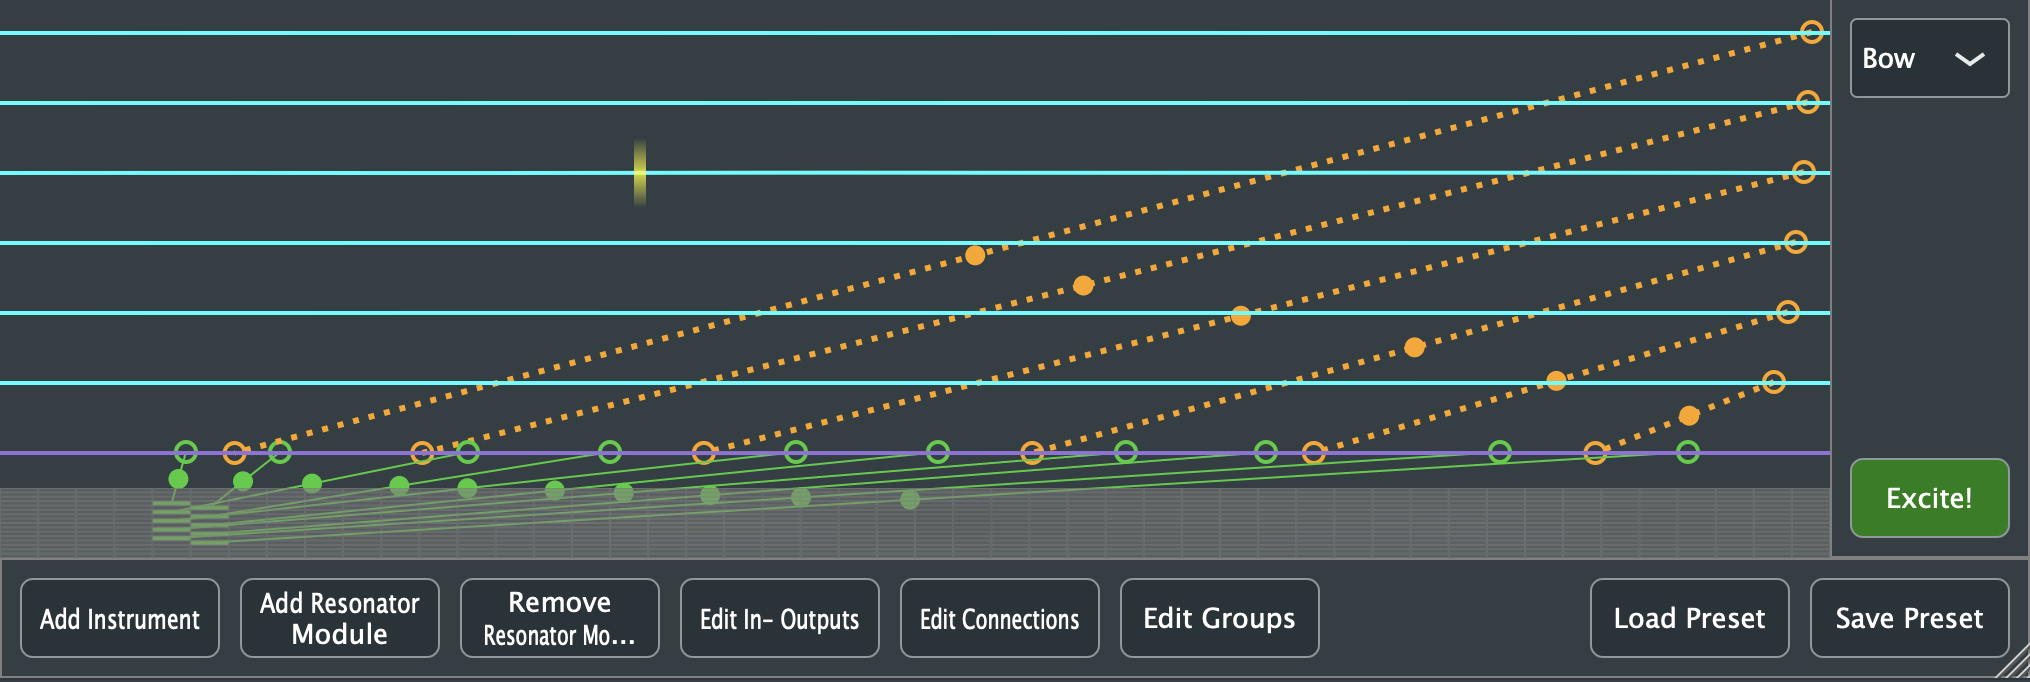
\includegraphics[width = \textwidth]{GUI.png}
    \caption{The graphical user interface (GUI) of the application presented in Section \ref{sec:application}. Here, the guitar preset is loaded with 6 strings, 1 bar, 1 thin plate and several linear (orange) and rigid (green) connections between them. The bowing excitation is chosen.}
    \label{fig:gui}
\end{figure*}
Introducing the centred difference and centred averaging operator
\begin{align}
    \dtd \eta^n &= \frac{1}{2k}\left(\eta^{n+1}-\eta^{n-1}\right)\approxeq \eta,\\
    \mtd \eta^n &= \frac{1}{2}\left(\eta^{n+1}+\eta^{n-1}\right)\approxeq \eta,
\end{align}
the spring in Eq. \eqref{eq:nonlinearSpring} can be discretised to
\begin{equation}\label{eq:nonlinearSpringDisc}
    f_\ctxt^n = K_{1,\ctxt}\mtd\eta_\ctxt^n + K_{3,\ctxt}(\eta_\ctxt^n)^2\mtd\eta_\ctxt^n + R_\ctxt\dtd \eta_\ctxt^n,
\end{equation}
which can be shown to be inherently stable \cite{theBible, Bilbao2009Modular}. The connection force can then be solved for according to
\begin{equation}\label{eq:springConnDisc}
    f_c^n = \frac{\eta_c^\star + \frac{\gamma_{c,-}}{\gamma_{c,+}}\eta_c^{n-1}}{\frac{1}{\gamma_{c,+}} + \frac{k^2}{a_{r_c}\mathcal{M}_{r_c}}+ \frac{k^2}{a_{s_c}\mathcal{M}_{s_c}}},
\end{equation}
where 
\begin{equation}
    \gamma_{c,\pm} = \frac{K_{1, c}}{2} + \frac{K_{3,c}(\eta_c^n)^2}{2} \pm \frac{R_c}{2k}.
\end{equation}
Notice that the rigid connection force in Eq. \eqref{eq:rigidConnDisc} is a special case of Eq. \eqref{eq:springConnDisc} where $\eta^{n-1}_c = 0$ and $\gamma_{c, +} \rightarrow \infty$. See \cite[Ch. 11]{WillemsenThesis} for a derivation and more details.

\subsection{Excitations}\label{sec:discExcitations}
This section discretises the excitations found in Section \ref{sec:contExcitations}. 

\subsubsection{The Bow}
The discretisation of the friction model in Eq. \eqref{eq:bowForce} as well as its implementation using an iterative solver -- such as Newton-Raphson -- is well-covered in the literature (see e.g. \cite[Ch. 8]{WillemsenThesis}). The spatial Dirac delta function in Eq. \eqref{eq:bowDistribution} is discretised using cubic spreading operator $J_{p,3}(\chi_\itxt)$, rather than Eq. \eqref{eq:spreading}, for more accurate control. Its definition is also excluded here for brevity, but can be found in the literature \cite[Sec. 5.2.4]{theBible}.
% \begin{equation}\label{eq:cubicJ}
%     J_{p,3}(\chi_\itxt) = \frac{1}{h}\begin{cases}
%         -\alpha_\itxt (\alpha_\itxt-1)(\alpha_\itxt-2)/6, & p = p_\itxt-1,\\
%         (\alpha_\itxt-1)(\alpha_\itxt+1)(\alpha_\itxt-2)/2,  & p = p_\itxt,\\
%         -\alpha_\itxt (\alpha_\itxt+1)(\alpha_\itxt-2)/2, & p = p_\itxt + 1,\\
%         \alpha_\itxt (\alpha_\itxt+1)(\alpha_\itxt-1)/6, & p = p_\itxt + 2,\\
%         0, & \text{otherwise.}
%     \end{cases}
% \end{equation}
% where $p_\itxt = \floor[\chi_\itxt / h]$ and $\alpha_\itxt = \chi_\itxt /h - p_\itxt$.

\subsubsection{Hammer and Pluck}
The discrete-time definition of Eq. \eqref{eq:massSpring} will not be given here. The discretisation of a mass-spring system can be found in e.g. \cite{Bilbao2009Modular, Willemsen2020}, and a derivation of the collision between the mass-spring and a 1D system using the non-iterative collision method used here (from \cite{Ducceschi2021}) is given in \cite[Sec. 10.2]{WillemsenThesis}.

For the pluck, $\tau$ will be set to 0 if $|f_\etxt / h| > \varphi$, where $\varphi$ is a threshold, which simulates a plucking interaction. Note that the force is scaled by the grid spacing of the respective resonator module so that the plucking interaction will be similar for strings with different parameters (and thus different values of $h$). 

\section{Real-Time Application}\label{sec:application}
A real-time application implementing the models above has been created in C++ using the JUCE framework\footnote{\url{https://juce.com}}. Figure \ref{fig:gui} shows the graphical user interface of the application using the guitar preset for illustration. The application is controlled using the mouse, and is divided into three main parts: the control panel (bottom), the excitation panel (right), and the instrument area. The latter is vertically and equally subdivided over the amount of instruments in the application, which in turn are subdivided vertically and equally into the amount of resonators they contain. The instrument area has a refresh rate of 15 Hz and visualises the states of the various resonator and exciter modules.  

After describing the system architecture, this section will go into detail of the functionality of the application.
An extensive demo of the application, going through all of the functionality described in this section, can be found via \cite{demo}.

\subsection{System Architecture}
Figure \ref{fig:systemArchitecture} illustrates the architecture of the audio-generating part of the application. The application can contain several independent instruments, each of which can contain several resonators. Furthermore, instruments contain information about the connections between various resonators. Every 1D resonator has three exciter modules, one for each of the excitations described in this paper. Only one of the exciter modules is activated at a time, controlled by the excitation panel (see Section \ref{sec:excitationPanel}). 
\begin{figure}[h]
    \centering
    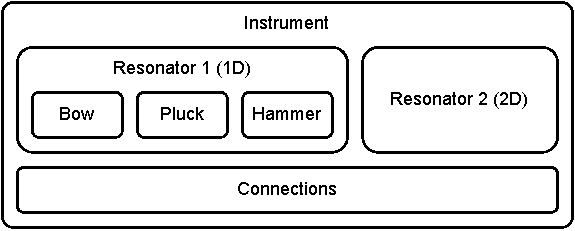
\includegraphics[width = \columnwidth]{systemArchitectureSMC2022.pdf}
    \caption{The system architecture. An instrument contains resonators as well as information about the connections between them. 1D resonators contain three exciter modules.}
    \label{fig:systemArchitecture}
\end{figure}

\subsection{Functionality}\label{sec:controlPanel}
This section goes through functionality of the application following the order of the various buttons shown in the control panel (bottom area in Figure \ref{fig:gui}).

\subsubsection{Instruments} 
The \textit{Add Instrument} adds an (additional) instrument to the application. Clicking on an instrument makes it the `currently active instrument' to which resonator modules can be added.

\subsubsection{Resonator Modules}\label{sec:resonatorModules}
The available resonators are: the stiff string, bar, membrane, thin plate and stiff membrane. The states of the 1D models are visualised as cyan (string) and purple (bar) lines and the states of 2D models as grey-scale squares (as done in e.g. \cite{Willemsen2019, Willemsen2020}).

The \textit{Add Resonator Module} button opens a window where a user can select a resonator type as well as its parameters. For the stiff string, one can choose an advanced (all parameters) and non-advanced (only the fundamental frequency and radius) list of parameters. For 2D models, an extra parameter `maxPoints' is given which alters the grid spacing such that the number of (moving) grid points does not surpass this. This is to not overload the CPU and keep the application running in real time. A button \textit{Add Module}, adds the resonator module to the currently selected instrument.

The \textit{Remove Resonator Modules} button changes the buttons in the control panel to \textit{Remove} and \textit{Done}. Clicking on a resonator module adds a red overlay, and clicking the \textit{Remove} button removes the resonator from the instrument.

It must be noted that if any button is pressed, the states of all resonator modules will be set to 0 to prevent audible artefacts when editing the settings. 


\subsubsection{Outputs}
The output of any model can be obtained by listening to $q_{\boldsymbol{l}_\text{o}}^n$ for an output location $\boldsymbol{l}_\text{o}$. In the application it is possible to change the output locations by clicking the \textit{Edit In- Outputs} button. If the button is clicked, the control panel will show instructions on the chosen option as well as a \textit{Done} button. The user can now add output locations to the various resonators. 

For 1D systems, outputs will show as downwards pointing arrows from the system state at the respective output locations. For 2D systems, rectangles around the output grid point are used. Left, right and stereo channels are shown in white, red and yellow respectively. Functionality to add inputs has been left for future work (see Section \ref{sec:conclusion}).

\subsubsection{Connections}\label{sec:connectionsApp}
Connections between resonators are visualised using coloured (dotted) lines (also see Figure \ref{fig:gui}). Rigid connections are shown in solid green, linear springs in dotted orange and non-linear springs in dotted magenta. A connection location on a 1D system is accentuated using a circle of the same colour, and the same is done for a 2D system using a rectangle. A solid circle along the connection line indicates the mass ratio between the grid points of the two components ($\mathcal{M}_{s_c} / \mathcal{M}_{r_c}$); the closer this is to one component, the heavier a grid point of that component is with respect to the other.  

If the \textit{Edit Connections} button is clicked, the control panel will change in the same way as for the \textit{Edit In- Outputs button}. Now, the currently active connection will be indicated by a yellow `halo' around the connection locations. If a user tries to overlap two connections, the currently active connection will be removed from the application.

\subsubsection{Groups}
If the \textit{Edit Groups} button is pressed, the control panel changes in the same way as for the previous two buttons.  The user can click on 1D resonator modules to add them to groups (see \cite{demo} for more details). Grouped models can be excited simultaneously (see Section \ref{sec:excitationPanel}).


\subsubsection{Presets}\label{sec:presets}
Presets are saved in `.xml' files and have the structure shown in Figure \ref{fig:presetStructure}. Each preset contains several elements (instruments, resonators, connections, etc.), each containing one or more attributes. 

Pressing the \textit{Load Preset} button causes a `File Chooser' window to pop up, where the user can select a local `.xml' file containing a preset. The \textit{Save Preset} button makes a window pop up with a text box into which the desired name of the current application configuration can be saved. If a file with that name already exists a warning window will pop up asking whether the existing file may be overwritten.

As different sample rates yield different values for $h$ (through Eq. \eqref{eq:stability}) and thus the number of grid points for each resonator, the locations of the outputs and connections are saved as ratios of the total number of grid points of the respective resonator. This allows the for the same relative locations of outputs and connections for one preset between different sample rates.

\begin{figure}[h]
    \centering
    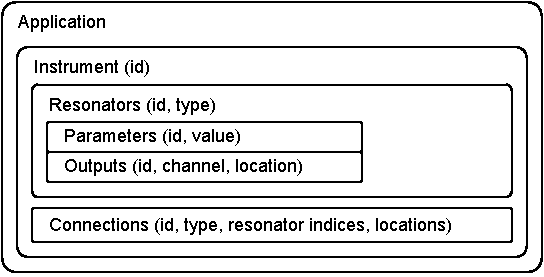
\includegraphics[width = \columnwidth]{presetStructure.pdf}
    \caption{Structure of the `.xml' files containing presets. Attributes for several elements are given in parentheses. %An application contains instruments which contain resonators and information on connections between them. The resonators contain parameters describing them as well as output locations.
    }
    \label{fig:presetStructure}
\end{figure}

\subsubsection{Excitations}\label{sec:excitationPanel}
One can interact with the various 1D resonator modules in the instrument area. The excitation panel (right area in Figure \ref{fig:gui}) contains a dropdown menu with the various excitations: \textit{Bow}, \textit{Hammer} and \textit{Pluck}. Selecting one of these activates the corresponding exciter module in all 1D resonator modules. Furthermore, an \textit{Excite!} button toggles the currently active exciter module for all 1D resonator modules. Now a user can hover the mouse over the resonator modules in the instrument area (or click for the hammer) to excite them. If the excitation is deactivated, all resonators (including 2D ones) can be excited using a raised cosine (although this is only used for testing purposes). Table \ref{tab:interactions} shows how the mouse is related to various excitation parameters.

\begin{table}[t]\label{tab:interactions}
\begin{center}
\begin{tabular}{|l|c|c|c|}
    \hline
    Mouse action & Bow & Hammer \& Pluck\\ \hline
    x-position & $\chi_\Btxt$& $\chi_\text{e}$ \\
    y-position & - & $z_\text{off}$ \\
    Scroll-wheel & $-0.2\leq v_\Btxt\leq 0.2$ & $ h \leq e_\text{w} \leq 10 h$\\
    Click & - & $\tau$ (hammer only) \\\hline
\end{tabular}
\caption{Mouse interactions related to the various excitations described in Section \ref{sec:excitationPanel}.}
\end{center}
\end{table}

The bow is visualised with a yellow rectangle with a moving gradient, the speed and direction of which depends on the value of the bow velocity ($v_\Btxt$ in Eq. \eqref{eq:vrel}). The mass used for the hammer and pluck ($z$ in Eq. \eqref{eq:massSpring}), is visualised using a yellow circle and follows the mouse / cursor. The excitation distribution ($e_\etxt$ in Eq. \eqref{eq:raisedCos}) is visualised using a grey ellipse around the cursor; its width is determined by the value of $e_\etxt$. For the hammer, a mouse click sets $\tau=0$ in Eq. \eqref{eq:massSpring}. If the hammer is triggered when the mass is further away from the string, the excitation will be of higher amplitude.

\subsection{Fixed parameters}\label{sec:fixedParams}
As described in Section \ref{sec:resonatorModules}, the parameters of the resonator modules can easily be altered by the user when adding one to the application. The parameters found in Table \ref{tab:parameters}, however, can not be altered by the user, and have been set to result in pleasing sounds for many different model configurations. Notice that the bow force is scaled by the values of $\rho$ and $A$ of the resonator module it is exciting so that bowing different strings will yield similar behaviour.
\begin{table}[t]\label{tab:parameters}
\begin{center}
\begin{tabular}{|l|c|c|}
    \hline
    Name & Symbol (unit) & Value\\ \hline
    \multicolumn{3}{|l|}{\bf Bow}\\ \hline
    Free parameter & $a_\Btxt$ (-) & $100$\\
    Bow force & $f_\Btxt$ (N) & $40 \cdot \rho A$\\\hline
    \multicolumn{3}{|l|}{\bf Hammer / pluck}\\ \hline
    Mass & $M_\text{z}$ (kg) & 0.01\\
    Spring coefficient & $K_\text{z}$ (N/m) & 1000\\
    Collision stiffness& $K_\etxt$ (N/m$^\alpha_\etxt$) & $10^6$\\
    Nonlin. coll. coeff. & $\alpha_\etxt$ (-) & 1.3\\
    Pluck force threshold & $\varphi$ (N/m) & 500\\\hline
    \multicolumn{3}{|l|}{\bf Connections}\\ \hline
    Linear spring coeff. & $K_1$ (N/m)  & $10^8$ \\
    Nonlin. spring coeff. & $K_3$ (N/m$^3$)  & $10^{10}$\\
    Damping coeff & $R$ (s$^{-1}$) & $0.01$
    \\\hline
\end{tabular}
\caption{List of fixed parameter values (see Section \ref{sec:fixedParams}).}
\end{center}
\end{table}

\section{Results and Discussion}\label{sec:resDiscuss}
Table \ref{tab:CPU} shows the CPU usage of the application with various settings and graphics turned off and on. Tests were carried out on a MacBook Pro with a 2,3 GHz Intel i9 processor. Results show that for many different configurations, the application is still able to run in real time (usage $<100\%$).

One can observe that the CPU increases with the number of grid points that need to be calculated per sample, which is an expected result. As more calculations need to be performed per sample for a 2D system the CPU usage is higher per grid point than for a 1D system. For two strings with all their moving grid points connected ($N=118$, $C=117$), the CPU usage increases significantly when compared to unconnected strings, and more so for non-rigid connections.

The graphics increase the CPU usage substantially, especially when connections need to be drawn. As the speed of the graphics thread has not been the focus during the development of the application, this could be optimised in the future. 

\begin{table}[t]
    \centering
    \begin{tabular}{|l|c|c|c|c|}
        \hline
    \multicolumn{5}{|l|}{\bf Strings ($N = 118$)}\\\hline
    No. of strings & 1 & 5 & 10 & 20 \\\hline
    No graphics & 1.7 & 7.4 & 12.3 &26.8\\
    Graphics & 8.3 & 14.0  & 19.4 & 35.0\\\hline
    \multicolumn{5}{|l|}{\bf Plate}\\\hline
    Moving points & 100 & 400 & 1600 & 2500 \\\hline
    No graphics & 4.8 & 15.4 & 47.0 & 63.3 \\
    Graphics & 12.0 & 23.9 & 59.2 & 77.5\\\hline
    \multicolumn{5}{|l|}{\bf Two connected strings ($N=118$, $C=117$)}\\\hline  
    Type & None & Rigid & Linear & Nonlinear \\\hline
        No graphics & 3.8 & 8.3 & 13.1 & 13.3\\
        Graphics & 12.7 & 28.4 & 42.3 & 43.1\\\hline
    \end{tabular}
    \caption{CPU usage (in \%) of the application with various configurations, and graphics turned on and off. }
    \label{tab:CPU}
\end{table}


% Right now, changes between sample rates are not included in the functionality of the application. As the sample rate is linked to the number of grid points, the locations of the outputs and connections are not included in the   the presets assume a sample

As mentioned in Section \ref{sec:connectionsApp}, overlapping connections are not possible in the current work. Although experiments with overlapping connections have been done, it has been decided to exclude these from the application. Following \cite{Bilbao2009Modular}, although any number of overlapping connections can be explicitly calculated, one needs to perform a matrix inversion every sample. Therefore, it was decided to exclude overlapping connections from the application. 

As mentioned in Section \ref{sec:introduction}, this application is part of a larger project, where will be used as a sound engine for a VR application. Hence, no usability tests have been performed, and are saved for the final product.

% To the best of the authors' knowledge, the way of real-time interactive excitation used for the hammer and the pluck applied to FDTD schemes has not been done before. %\SWcomment[@stefania, is this true? And should this be here?]

\section{Conclusion}\label{sec:conclusion}
This paper presented an application implementing various resonator modules using FDTD schemes which can be connected in a modular fashion to create (non)existing musical instruments. The instruments can be played in real time using bowing, hammering and plucking excitations.

Future work includes adding a greater variety of resonator modules (such as acoustic tubes) to the application, as well as applying the excitations presented here to 2D systems. It might also be interesting to explore the ability to add inputs to the resonator modules so that the application can be used as an audio effect. 
Finally, the authors would like to implement this system into a VR application where users will be able to build and play instruments in a virtual environment. 

\begin{acknowledgments}
This work has been funded in part by the European Art-Science-Technology Network for Digital Creativity (EASTN-DC), project number 883023.
\end{acknowledgments} 

%%%%%%%%%%%%%%%%%%%%%%%%%%%%%%%%%%%%%%%%%%%%%%%%%%%%%%%%%%%%%%%%%%%%%%%%%%%%%
%bibliography here
{\small
\bibliography{smc2022bib}
}
\end{document}
